\documentclass[crop=false,10pt]{standalone}
\usepackage{standard}

\begin{document}
  \section{Implementation} % (fold)
  \label{sec:Implementation}
    \begin{figure*}
      \center
      \begin{subfigure}[b]{0.49\textwidth}
        \center
        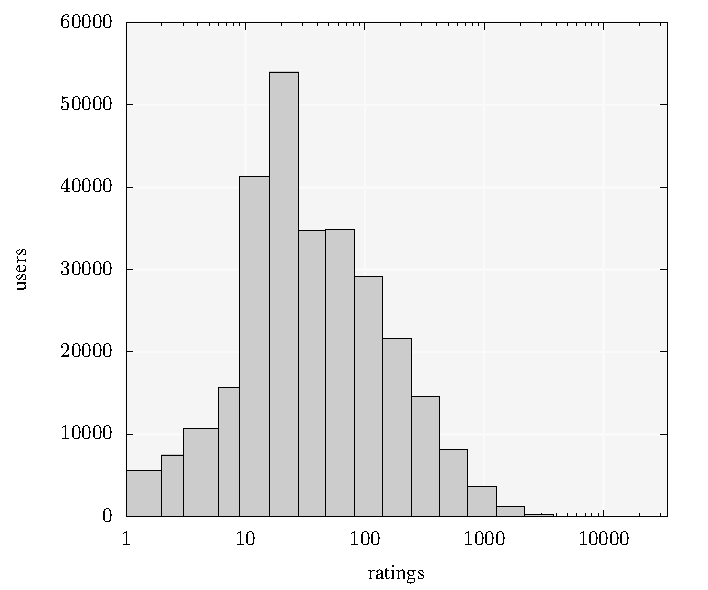
\includegraphics[width=0.99\textwidth]{figures/movielens-user-histogram.pdf}
      \end{subfigure}
      \hfill
      \begin{subfigure}[b]{0.49\textwidth}
        \center
        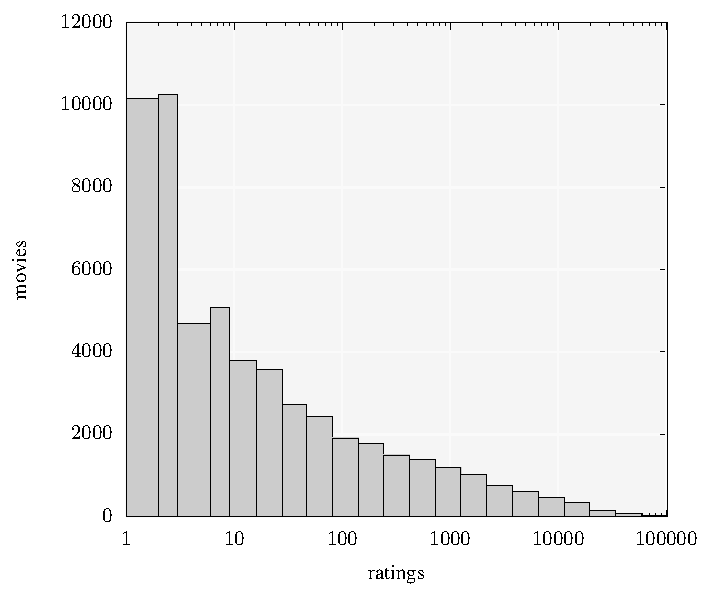
\includegraphics[width=0.99\textwidth]{figures/movielens-movie-histogram.pdf}
      \end{subfigure}
      \caption{%
        The figure shows two histograms for the latest MovieLens dataset \cite{MovieLensDataset}.
        The left one displays the counts of users over the number of ratings they have given to movies.
        The right one displays the counts of movies over the number of ratings they have received by users.
        It becomes clear that the matrix of ratings is a sparse matrix with no special structure.
      }
      \label{fig:rating-histograms}
    \end{figure*}

    To gather some ideas about the implementation of an RBM for collaborative filtering we will first examine some real dataset for movie ratings.
    This will give us an impression of problems and on what to focus when implementing the code in C++.
    For such investigations the latest MovieLens dataset \cite{MovieLensDataset} seems to be appropriate.
    It contains about 27,000,000 ratings for nearly 58,000 movies made by around 280,000 users.

    Before reading those ratings and writing them into a big matrix, like it was done in the example from table \ref{tab:problem-example}, we will take a look at the histograms in figure \ref{fig:rating-histograms} I have generated from this dataset.
    Here it becomes clear that most of the users have given something between 10 and 100 ratings to movies.
    There are some outliers.
    But even they could not give every available movie a rating.
    The same is true if we look at the histogram for movies.
    There are a lot of movies with a really small rating count.
    Hence, if we would generate a big matrix of ratings as in table \ref{tab:problem-example} most of the cells would contain $\times$ and would therefore be empty.
    This means that the matrix of ratings is really sparse without any given structure.
    It would be a waste of memory to use a dense matrix format to save and work with the ratings.

    As a consequence a sparse matrix format should be used.
    A typical and efficient suggestion is the compressed sparse row format (CSR).
    According to \cite{Bell2008} and \cite{Bell2009} it seems to be one of the best suited formats for this kind of problem.
    Matrix-vector multiplication in CSR can be implemented in parallel on CPUs and modern GPUs using CUDA.
    Typically, one does not like to implement such a low-level structure by hand.
    As an alternative one could use the format provided by the linear algebra libary \enquote{Eigen} \cite{eigen2018}.
    \cite{Bell2008,Bell2009}

    But reading the dataset of ratings presents us now with another problem.
    One user can give ratings to different movies and movies will receive different ratings from different users.
    Talking in the senses of relational databases the rating dataset can be described as an $n$-to-$m$ connection.
    Users and movies are typically referenced by some magic identification number which cannot be used as index for a vector or a matrix.
    This means while reading the dataset we have to keep track of unique users and unique movies by their identification number.
    Afterwards we have to be able to map these numbers to the indices of our rating matrix in both directions.
    The most efficient solution is to save pairs of identification numbers and indices inside a hash map.
    This will make sure every identification number is only inserted once and can be accessed in constant time complexity on average.
    Based on this hash map we can then generate a data vector of identification numbers with their position to be the index saved in the hash map.

    Until now we always assumed the values of the ratings to be binary.
    In reality those values most of the time have a small discrete set of values like $\set{1,2,3,4,5}{}$.
    This difference can be taken into account by mapping those values to $0$ or $1$.
    But in reality this is a poor approximation because we loose a lot information by doing this.
    A much more robust method is given by the usage of categorical RBMs which keep the main structure of a binary RBM but allow the visible values to be elements of a finite set of values.
    \cite{Hinton2007,Hinton2010,Murphy2012,towardsdatascience}

    Additionally, one should think of representing rating values as floating point types in C++.
    This approach will of course use much more memory.
    But we have got back a lot of memory by using a sparse matrix format.
    Using this memory for the floating points types will speed up the complete computation because we do not have to cast small integers to floating point values and vice versa.

    In section \ref{sec:Learning} we made clear that we will use one RBM for every user and that their weights and biases are connected.
    But in the end this was done from the abstract point of view of mathematical theory.
    Implementing one RBM for every user and connecting them somehow introduces an enormous overhead to the computation.
    But here the sparse matrix format comes in handy.
    We will only store one RBM in memory because weights and biases are connected anyway.
    The learning process on the other hand can be done independently for every user by using the entries in the sparse matrix of ratings directly.

    If we want to learn an RBM based on some ratings then afterwards we need to test the learned parameters by some test dataset.
    \cite{towardsdatascience} gives us a simple and robust method to do this with the MovieLens dataset \cite{MovieLensDataset}.
    It seems to be useful to use the complete user dataset in the training and test dataset.
    Hence, one should only divide the ratings of users into training and test dataset.
    \cite{towardsdatascience}
  % section Implementation (end)
\end{document}